\documentclass[11pt,letterpaper]{article}
\usepackage[lmargin=1in,rmargin=1in,tmargin=1in,bmargin=1in]{geometry}
\usepackage{../style/homework}
\usepackage{../style/commands}
\setbool{quotetype}{false} % True: Side; False: Under
\setbool{hideans}{false} % Student: True; Instructor: False

% -------------------
% Content
% -------------------
\begin{document}

\homework{10: Due 04/27}{An approximate answer to the right problem is worth a good deal more than an exact answer to an approximate problem.}{John Tukey}

% Problem 1
\problem{10} Find the least square regression line, along with the $r$ and $r^2$ value, for the dataset $\{ (-1, -2), (1, 3), (2, 2), (4, 5) \}$. Show all your work. \pspace

\sol We have 4 points so that $n= 4$. First, we compute the $x$ and $y$ averages---$\overline{x}$ and $\overline{y}$, respectively. 
	\[
	\begin{aligned}
	\overline{x}&= \dfrac{\sum x_i}{n}= \dfrac{-1 + 1 + 2 + 4}{4}= \dfrac{6}{4}= 1.5 \\
	\overline{y}&= \dfrac{\sum y_i}{n}= \dfrac{-2 + 3 + 2 + 5}{4}= \dfrac{8}{4}= 2.00 
	\end{aligned}
	\]
Now we compute $s_x, s_y, r$:
	\begin{table}[!ht]
	\centering
	\begin{tabular}{rrrrrr}
	$x$ & $y$ & $x_i - \overline{x}$ & $(x_i - \overline{x})^2$ & $y_i - \overline{y}$ & $(y_i - \overline{y})^2$ \\ \hline
	$-1$ & $-2$ & $-2.5$ & $6.25$ & $-4$ & $16$ \\ 
	$1$ & $3$ & $-0.5$ & $0.25$ & $1$ & $1$ \\
	$2$ & $2$ & $0.5$ & $0.25$ & $0$ & $0$ \\
	$4$ & $5$ & $2.5$ & $6.25$ & $3$ & $9$ \\ \hline
	& Total: & & $13.00$ & & $26$ 
	\end{tabular}
	\end{table}
Then we have
	\[
	\begin{aligned}
	s_x^2&= \dfrac{1}{n - 1} \sum (x_i - \overline{x})^2= \dfrac{1}{4 - 1} \cdot 13.00= 4.3333 \Longrightarrow s_x= \sqrt{4.3333}= 2.0817 \\
	s_y^2&= \dfrac{1}{n - 1} \sum (y_i - \overline{y})^2= \dfrac{1}{4 - 1} \cdot 26= 8.6667 \Longrightarrow s_y= \sqrt{8.6667}= 2.9439
	\end{aligned}
	\]
Now we also compute the $r$ value:
	\begin{table}[!ht]
	\centering
	\begin{tabular}{rrrrrrr}
	$x$ & $y$ & $x_i - \overline{x}$ & $\frac{x_i - \overline{x}}{s_x}$ & $y_i - \overline{y}$ & $\frac{y_i - \overline{y}}{s_y}$ & $\frac{x_i - \overline{x}}{s_x} \cdot \frac{y_i - \overline{y}}{s_y}$ \\ \hline
	$1$ & $1$ & $-2.5$ & $-1.2009$ & $-4$ & $-1.3587$ & $1.6317$ \\ 
	$1$ & $0$ & $-0.5$ & $-0.2402$ & $1$ & $0.3397$ & $-0.0816$ \\
	$2$ & $3$ & $0.5$ & $0.2402$ & $0$ & $0.0000$ & $0.0000$ \\
	$3$ & $4$ & $2.5$ & $1.2009$ & $3$ & $1.0191$ & $1.2238$ \\ \hline
	& Total: & &  & & & $2.7739$
	\end{tabular}
	\end{table}
	\[
	r= \dfrac{1}{n - 1} \sum \left( \dfrac{x_i - \overline{x}}{s_x} \right) \left( \dfrac{y_i - \overline{y}}{s_y} \right)= \dfrac{1}{4 - 1} \cdot 2.7739= 0.9246
	\]
Therefore, $r^2= 0.8549$. Finally, we can compute our regression coefficients:
	\[
	b_1= r\, \dfrac{s_y}{s_x}= 0.9246 \cdot \dfrac{2.9439}{2.0817}= 1.308 \quad \text{ and } \quad b_0= \overline{y} - b_1 \overline{x}= 2.00 - 1.308 \cdot 1.5= 0.038
	\]
Therefore, as $\widehat{y}= b_1x + b_0$, we know $\widehat{y}= 1.308x + 0.038$. 



\newpage



% Problem 2
\problem{10} Given the following information below, find the least square regression line. Show all your work. 
	\[
	\begin{aligned}
	n&= 10 \\
	\overline{x}&= 19.59, \quad s_x^2&= 2.9225 \\
	\overline{y}&= 15.63, \quad s_y^2&= 5.2407 \\
	R&= 0.8733
	\end{aligned}
	\] \pspace

\sol Because $s_x^2= 2.9225$ and $s_y^2= 5.2407$, we know that $s_x= \sqrt{2.9225}= 1.7095$ and $\sigma_y= \sqrt{5.2407}= 2.2893$. But then\dots
	\[
	\begin{aligned}
	b_1&= R\;\dfrac{s_y^2}{s_x^2}= 0.8733\; \dfrac{2.2893}{1.7095}= 1.1695 \\[0.3cm]
	b_1&= \overline{y} - b_1 \overline{x}= 15.63 - 1.1695 \cdot 19.59= -7.2805
	\end{aligned}
	\] \pvspace{0.3cm}
Therefore, as $\widehat{y}= b_1x + b_0$, we know that $\widehat{y}= 1.1695x - 7.2805$. 



\newpage



% Problem 3
\problem{10} Match each regression coefficient to its corresponding graph. 
	\begin{figure}[!ht]
	\centering
	\begin{minipage}{0.45\textwidth}
	   \centering
	   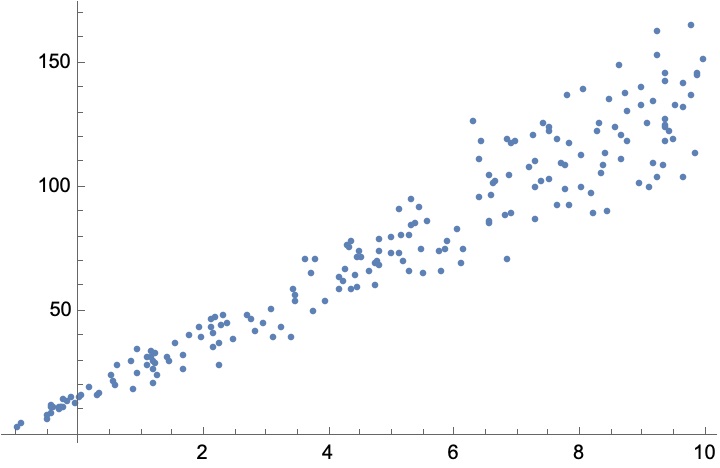
\includegraphics[width=0.9\textwidth]{reg1.png}
	   \caption*{(a)}
	\end{minipage}\hfill
	\begin{minipage}{0.45\textwidth}
	   \centering
	   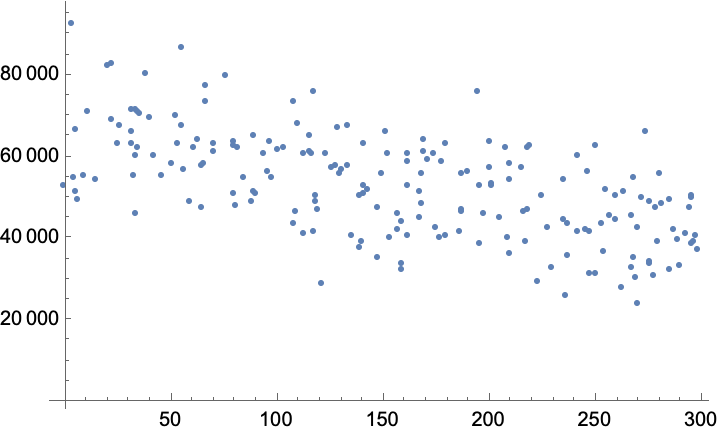
\includegraphics[width=0.9\textwidth]{reg2.png}
	   \caption*{(b)}
	\end{minipage}
	\begin{minipage}{0.45\textwidth}
	   \centering
	   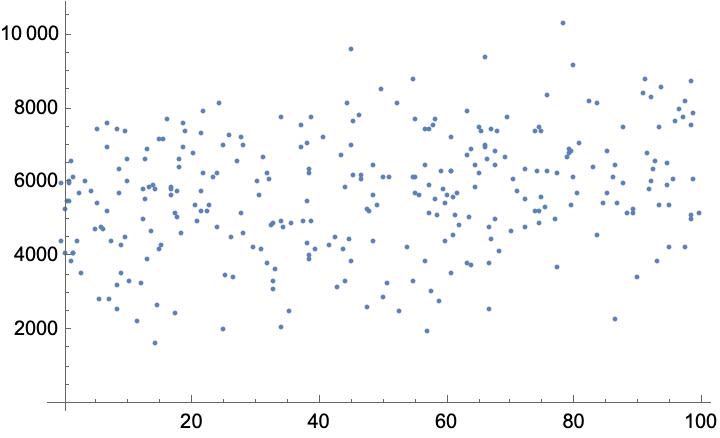
\includegraphics[width=0.9\textwidth]{reg3.png}
	   \caption*{(c)}
	\end{minipage}
	\begin{minipage}{0.45\textwidth}
	   \centering
	   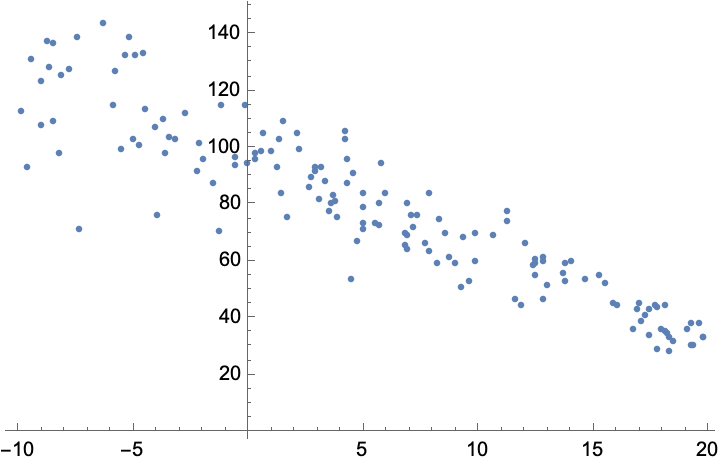
\includegraphics[width=0.9\textwidth]{reg4.png}
	   \caption*{(d)}
	\end{minipage}
	\end{figure}

\begin{enumerate}[(i)]
\item\underline{\hspace{0.5cm}(d)\hspace{0.5cm}}: $R= -0.9197$
\item\underline{\hspace{0.5cm}(b)\hspace{0.5cm}}: $R= -0.6023$
\item\underline{\hspace{0.5cm}(c)\hspace{0.5cm}}: $R= 0.2527$
\item\underline{\hspace{0.5cm}(a)\hspace{0.5cm}}: $R= 0.9616$
\end{enumerate} 



\newpage



% Problem 4
\problem{10} A researcher is trying to predict home run records. The researcher wants to predict what the next home run record will be. To model this, they will take the last ten home run records and label them as $r= 1, 2, \ldots, 10$, i.e. $r= 1$ is the tenth highest home run record, $r= 2$ is the ninth highest home run record, etc.. They fit a linear regression to this data and find a simple linear regression model of $h(r)= 20.21r + 559.3$. 
	\begin{enumerate}[(a)]
	\item What are $b_0$ and $b_1$ for this linear regression?
	\item Predict the future home run record by finding $h(11)$.
	\item For $r= 8$, the home run record, $h(8)$, was known to be Babe Ruth's record of 714 home runs. Find the residual for this value given the model.
	\item The researcher finds an $R^2$ value of $0.9837$. Is the linear model a good fit to the home run record data? Explain. 
	\end{enumerate} \pspace

\sol 
\begin{enumerate}[(a)]
\item We know that a simple linear regression is of the form $\widehat{y}= b_1 x + b_0$. because we have $h(r)= 20.21r + 559.3$, we have $b_1= 20.21$ and $b_0= 559.3$. \pspace

\item We have\dots
	\[
	h(11)= 20.21(11) + 559.3= 222.31 + 559.3= 781.61
	\] \pspace

\item We have\dots
	\[
	h(8)= 20.21(8) + 559.3= 161.68 + 559.3= 720.98
	\]
Therefore, the residual is $e= y - \widehat{y}= 714 - 720.98= -6.98$. \pspace

\item Because $R^2= 0.9837 > 0.85$, this is a `good' fit for the data. Because $R^2= 0.9837$, 98.37\% of the variation in the home runs is explained by the model. 
\end{enumerate}


\end{document}